\section{Project implementation}


\begin{frame}
\frametitle{Project overview}
\begin{figure}[htbp]
   \centering
   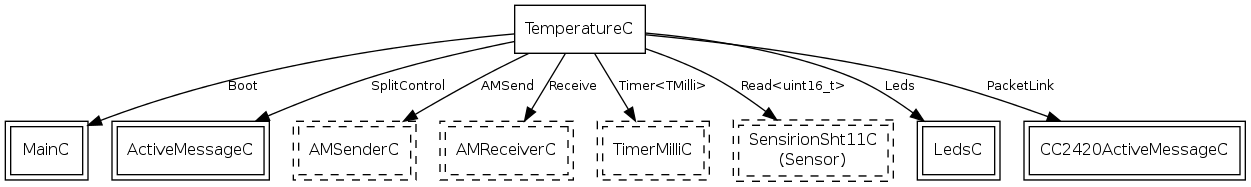
\includegraphics[width=\textwidth]{img/TemperatureAppC.png} 
\end{figure}

\end{frame}

\begin{frame}
\frametitle{Temperature measuring}
The conversion given a digital readout ($SO_{T}$) to a temperature value is given at the following formula:
\begin{align*}
	T &= d_{1} + d_{2} \cdot SO_{T}
\end{align*}
where the coefficients is the following
\begin{table}[ht]
\centering
\begin{tabular}{ | l | c | r | }
	\hline
	VDD & $d_{1} \ ^{\circ}  C$ & $d_{1} \ ^{\circ}  F$ \\
	\hline \hline
	5V & -40.1 & -40.2 \\
	\hline
	4V & -39.8 & -39.6 \\
	\hline
	3.5V & -39.7 & -39.5 \\
	\hline
	3V & -39.6 & -39.3 \\
	\hline
	2.5V & -39.4 & -38.9 \\
	\hline
\end{tabular}
\begin{tabular}{ | l | c | r | }
	\hline
	$SO_{T}$ & $d_{2}  \ ^{\circ}C$ & $d_{2} \ ^{\circ} F$ \\
	\hline \hline
	14 bit & 0.01 & 0.018 \\
	\hline
	12 bit & 0.04 & 0.072\\
	\hline
\end{tabular}
\caption{Temperature conversion coefficients}
\label{table:temperature}
\end{table}

\end{frame}

\begin{frame}[fragile]
\frametitle{Package ACK with PacketAcknowledgements interface}
\begin{lstlisting}[caption={TemperatureAppC.nc}]
 TemperatureC.PacketAcknowledgements -> ActiveMessageC;
\end{lstlisting}


\begin{lstlisting}[caption={TemperatureC.nc $\rightarrow$ sendReadings()}]
memcpy(call AMSend.getPayload(&sendBuf, sizeof(local)),
    &local, sizeof local);
call PacketAcknowledgements.requestAck(&sendBuf);
if (call AMSend.send(SINK_NR, &sendBuf, sizeof local)
    == SUCCESS) {
    sendBusy = TRUE;
    ackTries++;
}
\end{lstlisting}

\end{frame}

\begin{frame}[fragile]
\frametitle{Package ACK with PacketAcknowledgements interface}

\begin{lstlisting}[caption={TemperatureC.nc $\rightarrow$ AMSend.sendDone()}]
if(call PacketAcknowledgements.wasAcked(msg)) {
    reportSent();
    ackTries = 0;
} else {
    if (ackTries < NACKTRIES) {
        sendReadings();
    } else if (ackTries == NACKTRIES) {
        ackTries = 0;
        sleep();
    }
}
\end{lstlisting}

\end{frame}

\begin{frame}[fragile]
\frametitle{Package ACK with PacketLink interface}
\begin{lstlisting}[caption={TemperatureAppC.nc}]
TemperatureC.PacketLink -> CC2420ActiveMessageC;
\end{lstlisting}

\begin{lstlisting}[caption={TemperatureC.nc $\rightarrow$ sendReadings()}]
memcpy(call AMSend.getPayload(&sendBuf, sizeof(local)),
    &local, sizeof local);
call PacketLink.setRetries(&sendBuf, 10);
call PacketLink.setRetryDelay(&sendBuf, 500);
if (call AMSend.send(SINK_NR, &sendBuf, sizeof local)
    == SUCCESS) {
    sendBusy = TRUE;
}
\end{lstlisting}

\end{frame}

\begin{frame}[fragile]
\frametitle{Package ACK with PacketLink interface}

\begin{lstlisting}[caption={TemperatureC.nc $\rightarrow$ AMSend.sendDone()}]
if (call PacketLink.wasDelivered(msg)){
    reportSent();
    sleep();
} else {
    reportProblem();
    sleep();
}
\end{lstlisting}

\end{frame}

%%% Local Variables: 
%%% mode: latex
%%% TeX-master: "../presentation"
%%% End: 
